\documentclass{article}

\usepackage{color}
\usepackage{mathrsfs,amsmath}
\usepackage{xcolor}
\usepackage{titlesec}
\usepackage{listings}
\usepackage{syntax}
\usepackage{pythonhighlighting}
\usepackage{fancyvrb}
\usepackage{minted} 

\usepackage{graphicx}

\graphicspath{ {./assets/} }

\usepackage[margin=1.4in]{geometry}

\title{Homework \#3 | Fall 2021} 
\author{Jared Dyreson\\ 
        California State University, Fullerton}

\DeclareRobustCommand{\bowtie}{%
  \mathrel\triangleright\joinrel\mathrel\triangleleft}



\definecolor{mygray}{rgb}{0.4,0.4,0.4}
\definecolor{mygreen}{rgb}{0,0.8,0.6}
\definecolor{myorange}{rgb}{1.0,0.4,0}

\usepackage [english]{babel}
\usepackage [autostyle, english = american]{csquotes}
\MakeOuterQuote{"}

\titlespacing*{\section}
{0pt}{5.5ex plus 1ex minus .2ex}{4.3ex plus .2ex}
\titlespacing*{\subsection}
{0pt}{5.5ex plus 1ex minus .2ex}{4.3ex plus .2ex}

\usepackage{hyperref}
\hypersetup{
    colorlinks,
    citecolor=black,
    filecolor=black,
    linkcolor=black,
    urlcolor=black
}

\begin{document}

\maketitle
\tableofcontents

\newpage

\section{General Information}

\subsection{Contributors}

\begin{enumerate}
\item Jared Dyreson | \href{mailto:jareddyreson@csu.fullerton}{\underline{jareddyreson@csu.fullerton.edu}} | CWID: 889546529
\end{enumerate}

\subsection{Repository}

The repository for this project can be found \href{https://github.com/JaredDyreson/CS335_Project3}{\underline{here}}. Please consult the README.md file for more information regarding the execution of the program.

\newpage

\section{Algorithm 1 | Pattern Sorting}

\subsection{Pseudocode}

\begin{verbatim}

function swap(a: int, b: int):
    c: int = a
    a = b
    b = c

function pattern_sorting(container: list[int], pattern: list[int]):
    for key in pattern:
        for i in range(0, container.size()):
            for j in range(i, container.size()):
                if(key == container[i]):
                    swap(container[i], container[j])
\end{verbatim}

\subsection{Mathematical Analysis}

In this function, we need to rearrange the array based on a pattern that contains at least one element in the aforementioned array.
To begin, you need to iterate over all the keys to sort once, which will be linear time $O(n)$.
For this routine, you will need a nested for loop to check the current index to all of the neighboring indices. That inner loop takes $O(n^{2})$.
This sorting algorithm takes directly from bubble sort, where the swap takes place when we meet the criteria.
In this instance, the criteria is the left hand side of the array's index being equal to the current value in the pattern.
In terms of memory usage, the only other external data container is a single integer in the swap method. Other than that, the program uses no extra space when sorting.
We can come to the conclusion that since the outermost loop of $O(n)$ needs to run $O(n^{2})$ times per iteration, the running time complexity is $O(n^{3})$.

\newpage

\section{Algorithm 2 | Merging Arrays}

\subsection{Pseudocode}

\begin{verbatim}
function merge(input: list[list[int]]):
    heap = createHeap(int, list[int], lessThanComp) # O(n)

    # nested loops are O(log(n) * n^2)
    for row in input: 
        for element in row:
            heap.insert(element)

    external: list[int] = []  # O(1)

    while heap is not empty: # O(log(n))
        external.append(heap.pop())
        
\end{verbatim}

\subsection{Mathematical Analysis}

In this function, we need to merge a collection of arrays into one large array and the resultant must be sorted in descending order.
To achieve this, we are going to employ a min heap and it uses a priority queue with a greater than comparator to sort them.
Here is an example of what min heap looks like; the least most element is at the top and removal of the root will have the least most element bubble to the top.

\begin{figure}[!h]
\centering
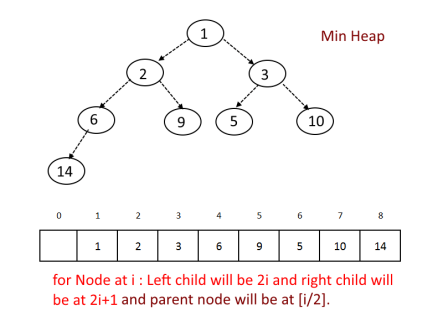
\includegraphics[width=9cm]{min_heap}
\end{figure}

First, creating a min heap will take $O(n)$ time and will use a list to store all the values in the tree.
Then, we need to iterate over the collection of arrays that contain the data we need to sort.
This takes $O(n^{2})$ time because of the way the data is stored. 
If the data was stored in a contiguous data structure, this would only take $O(n)$ time but will still result in around the same amount of time as the number of elements hasn't changed.
Each insertion inside the min heap will take $O(\log(n))$ time.
Lastly, extracting the data from the heap will take $O(\log(n))$ per instance, it should be around $O(n)$ because we're completely emptying the heap.
Overall, the time complexity for this function should be $O(\log(n) * n^{2})$.

\end{document}
